\documentclass[11pt]{article}
\usepackage{tikz}
\usetikzlibrary{decorations.pathreplacing,calligraphy}
\usetikzlibrary{calc}
\usetikzlibrary{shapes.geometric}
\usetikzlibrary{arrows.meta}
\usepackage[utf8]{inputenc}
\usepackage[T1]{fontenc}
\usepackage{textcomp,amssymb,amsmath,amsthm}
\usepackage{xcolor}
\tikzset{sttriangle/.style={
    draw=black,
    fill=white,
    regular polygon,
    regular polygon sides=3,
    minimum size = 0pt,
    inner sep=1pt
}}
\tikzset{stcircle/.style={
    fill=white,
    draw=black,
    circle,inner sep=1pt,
    minimum size = 1.5em
}}
\tikzset{rednode/.style={
    fill=white,
    draw=black,
    circle,
    inner sep=1pt,
    minimum size = 1.5em
}}
\tikzset{blacknode/.style={
    text=white,
    fill=black,
    draw=black,
    circle,
    inner sep=1pt,
    minimum size = 0.5em
}}
\tikzset{splitter/.style={
    fill=black,
    circle,
    inner sep=0pt,
    minimum size = 4pt
}}
\tikzset{term/.style={
    draw=black,
    fill=black,
    rectangle,
    inner sep=0pt,
    minimum size=4pt
}}
\tikzset{chooser/.style={
    draw=black,
    fill=white,
    circle,
    inner sep=0pt,
    minimum size = 4pt
}}
\tikzset{saturated/.style={very thick}}
\tikzset{fluid/.style={}}
\tikzset{OutPrio/.tip = {||.}}

\begin{document}

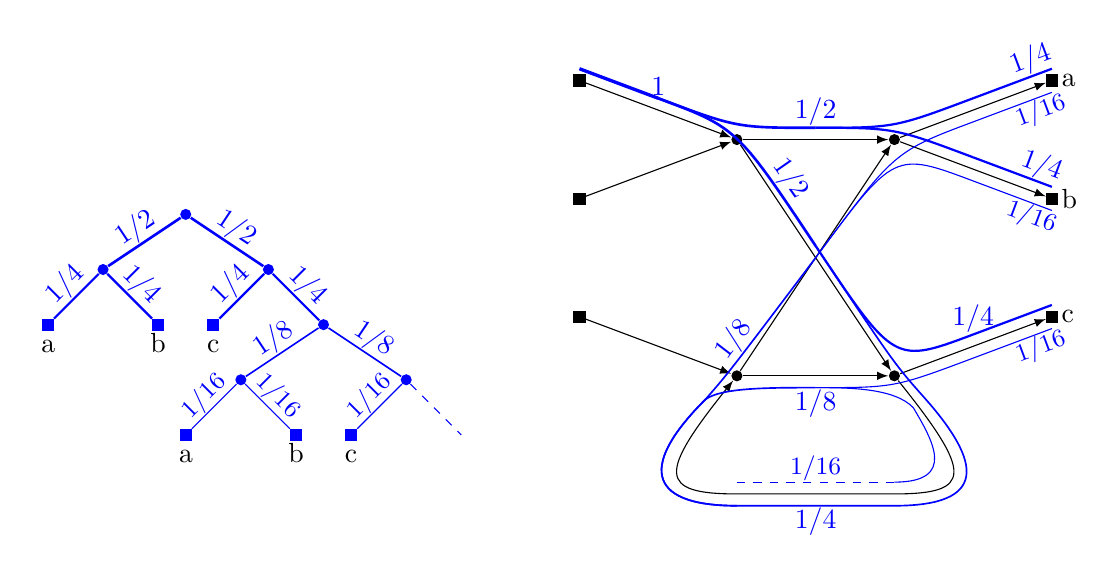
\begin{tikzpicture}[x=2cm,y=1.5cm,>=latex]
  \foreach \n in {1,2,3} {
    \node[term] (i\n) at (0,\n) {}; 
    \node[term] (o\n) at (3,\n) {};
  }
  \foreach \n/\x/\y in {a/1/0.5,b/1/2.5,c/2/0.5,d/2/2.5} {
    \node[splitter] (\n) at (\x,\y) {};
  }
  \draw[->,fluid] (i1) -- (a);
  \draw[->,fluid] (i2) -- (b);
  \draw[->,fluid] (i3) -- (b);
  \draw[->,fluid] (a) -- (c);
  \draw[->,fluid] (a) -- (d);
  \draw[->,fluid] (b) -- (c);
  \draw[->,fluid] (b) -- (d);
  \draw[->,fluid] (c) -- (o1);
  \draw[->,fluid] (d) -- (o2);
  \draw[->,fluid] (d) -- (o3);
  \draw[->,fluid] (c) .. controls (2.5,-0.33) and (2.5,-0.5) .. (2,-0.5) 
  -- (1,-0.5) .. controls (0.5,-0.5) and (0.5,-0.33) .. (a);
  \draw[blue,very thick] ($(i3.center) + (0,0.1)$) 
  -- ($(0.5,2.75) + (0,0.1)$) node[above=-3pt] {$1$}; 
  \draw[blue,line width=0.95pt] ($(0.5,2.75) + (0,0.1)$)
  .. controls ($(b.center) + (0,0.1)$) 
  .. ($(1.5,2.5) + (0,0.1)$) node[above=-3pt] {$1/2$}; 
  \draw[blue,thick] ($(1.5,2.5) + (0,0.1)$) 
  .. controls ($(d.center) + (0,0.1)$) 
  .. ($(2.5,2.75) + (0,0.1)$);
  \draw[blue,thick] ($(2.5,2.75) + (0,0.1)$) 
  -- ($(o3.center) + (0,0.1)$) node[above=-3pt,sloped,pos=0.8] {$1/4$};;
  \draw[blue,thick] ($(1.5,2.5) + (0,0.1)$) 
  .. controls ($(d.center) + (0,0.1)$) 
  .. ($(2.5,2.25) + (0,0.1)$); 
  \draw[blue,thick] ($(2.5,2.25) + (0,0.1)$) 
  -- ($(o2.center) + (0,0.1)$) node[above=-3pt,sloped,pos=0.8] {$1/4$};
  \draw[blue,line width=0.95pt] ($(0.5,2.75) + (0,0.1)$) 
  .. controls ($(b.center) + (0,0.1)$) 
  .. ($(1.5,1.5) + (0,0.1)$) node[above=-3pt,sloped,pos=0.8] {$1/2$}; 
  \draw[blue,thick] ($(1.5,1.5) + (0,0.1)$) 
  .. controls ($(c.center) + (0,0.1)$)
  .. ($(2.5,0.75) + (0,0.1)$) node[above=-3pt] {$1/4$}; 
  \draw[blue,thick] ($(2.5,0.75) + (0,0.1)$) -- ($(o1.center) + (0,0.1)$);
  \draw[blue,thick] ($(1.5,1.5) + (0,0.1)$) 
  .. controls ($(c.center) + (0,0.1)$)
  .. (2.2,0.3)
  .. controls (2.55,0.-0.23) and (2.6,-0.6) .. (2,-0.6) 
  -- (1,-0.6) node[midway,below=-3pt] {$1/4$}
  .. controls (0.4,-0.6) and (0.4,-0.23) 
  .. (0.8,0.3) [semithick] 
  .. controls ($(a.center) + (-0.05,+0.03)$)
  .. ($(1.5,1.5)$) node[pos=0.6,above=-3pt,sloped] {$1/8$};
  \draw[blue,thick] (1,-0.6)
  .. controls (0.4,-0.6) and (0.4,-0.23)
  .. (0.8,0.3) [semithick]
  .. controls (0.9,0.4) and ($(a.center) + (0.2,-0.1)$) 
  .. ($(1.5,0.5) - (0,0.1)$) node[below=-3pt] {$1/8$};
  \draw[blue,thin] ($(1.5,1.5)$)
  .. controls ($(d.center) - (0,0.1)$) 
  .. ($(2.5,2.75) - (0,0.1)$) 
  -- ($(o3.center) - (0,0.1)$) node[pos=0.8,below=-3pt,sloped] {\small $1/16$}; 
  \draw[blue,thin] ($(1.5,1.5)$)
  .. controls ($(d.center) - (0,0.1)$) 
  .. ($(2.5,2.25) - (0,0.1)$) 
  -- ($(o2.center) - (0,0.1)$) node[pos=0.8,below=-3pt,sloped] {\small $1/16$}; 
  \draw[blue,thin] ($(1.5,0.5) - (0,0.1)$)
  .. controls ($(c.center) - (0,0.1)$) 
  .. ($(2.5,0.75) - (0,0.1)$)
  -- ($(o1.center) - (0,0.1)$) node[pos=0.8,below=-3pt,sloped] {\small $1/16$};
  \draw[blue,thin] ($(1.5,0.5) - (0,0.1)$)
  .. controls (1.7,0.4) and ($(c.center) - (0,0.1)$) %(2,0.4)
  .. (2.12,0.23)
  .. controls ($(2.24,0.06) - (0,0.1)$) and ($(2.4,-0.5) + (0,0.1)$) 
  .. ($(2,-0.5) + (0,0.1)$);
  \draw[blue,very thin,dashed] ($(2,-0.5) + (0,0.1)$)
  -- ($(1,-0.5) + (0,0.1)$) node[midway,above=-3pt,sloped] {\small $1/16$};
  \draw (o1) node[anchor=west] {c};
  \draw (o2) node[anchor=west] {b};
  \draw (o3) node[anchor=west] {a};
  \begin{scope}[xshift=-5cm,x=0.7cm,y=0.7cm]
    \foreach \n/\x/\y in {a/0/4,b/-1.5/3,c/1.5/3,g/2.5/2,h/1,i/4/1}
    {
      \node[splitter,blue] (\n) at (\x,\y) {};
    } 
    \foreach \n/\x/\y in {d/-2.5/2,e/-0.5/2,f/0.5/2,j/0/0,k/2/0,l/3/0}
    {
      \node[term,blue] (\n) at (\x,\y) {};
    } 
    \foreach \u/\v in {a/b,a/c} {
      \draw[blue,line width=0.95] (\u) -- (\v) node[sloped,midway,above=-3pt] {$1/2$};
    }
    \foreach \u/\v in {b/d,b/e,c/f,c/g} {
      \draw[blue,thick] (\u) -- (\v) node[sloped,midway,above=-3pt] {$1/4$};
    }
    \foreach \u/\v in {g/h,g/i} { 
      \draw[blue,semithick] (\u) -- (\v) node[sloped,midway,above=-3pt] {$1/8$};
    }
    \foreach \u/\v in {h/j,h/k,i/l} {
      \draw[blue,thin] (\u) -- (\v) node[sloped,midway,above=-3pt] {\small $1/16$};
    }

    \draw[blue,thin] (i) -- (4.5,0.5) [dashed] -- (5,0);
    \draw ($(d) - (0,1em)$) node[anchor=base] {a};
    \draw ($(e) - (0,1em)$) node[anchor=base] {b};
    \draw ($(f) - (0,1em)$) node[anchor=base] {c};
    \draw ($(j) - (0,1em)$) node[anchor=base] {a};
    \draw ($(k) - (0,1em)$) node[anchor=base] {b};
    \draw ($(l) - (0,1em)$) node[anchor=base] {c};
  \end{scope}
\end{tikzpicture}

\end{document}